\chapter{Markov Decision Processes}

MDPs are a classical formalization of sequential decision making, where actions influence not just immediate rewards but also subsequent situations or states, and through those future rewards. Whereas in bandit problems we estimated the value $q_*(a)$ of each action $a$, in MDPs we estimate the value $q_*(s,a)$ of each action $a$ in each state $s$, or we estimate the value $v_*(s)$ of each state given optimal action selections. 

\section{Interface}

The learner and decision maker is called the \textbf{agent}. The thing it interacts with, comprising everything outside the agent, is called the \textbf{environment}. These interact continually, the agent selecting actions and the environment responding to these actions and presenting new situations to the agent. The environment also gives rise to rewards, special numerical values that the agent seeks to maximize over time through its choice of actions. 

General scheme of a \textit{Decision Process}:

\begin{center}
    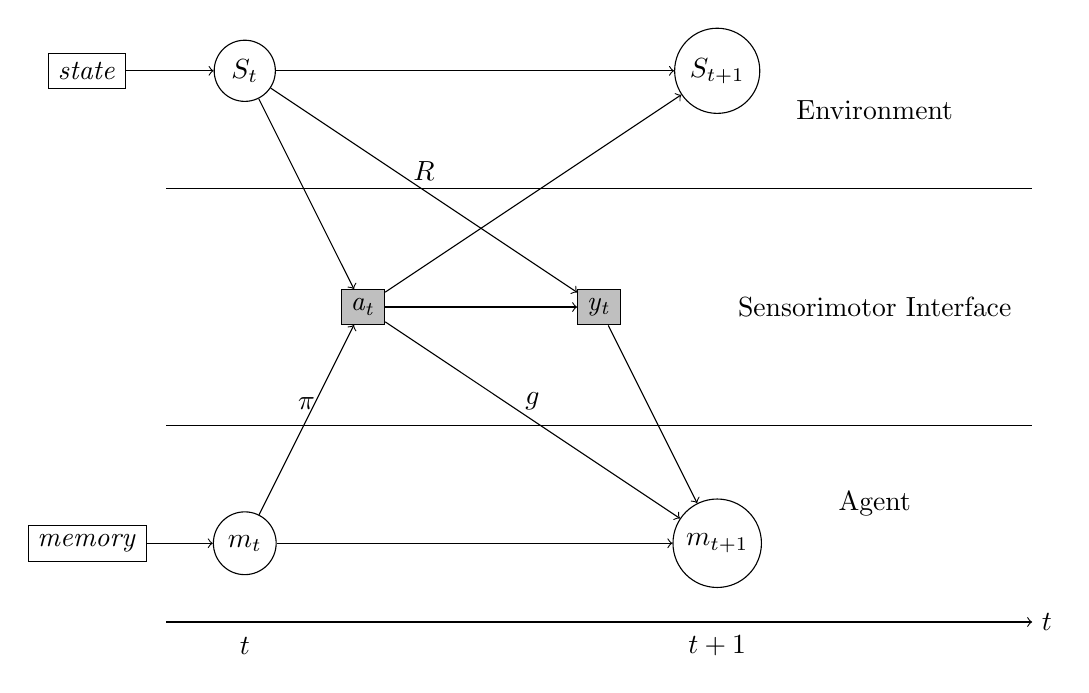
\begin{tikzpicture}

        % Time axis
        \draw[->] (-4, -4) -- (7, -4) node[right] {\(t\)};
        
        % Time labels
        \node at (-3, -4.3) {\(t\)};
        \node at (3, -4.3) {\(t+1\)};

        % Lines
        \draw (-4, -1.5) -- (7, -1.5) node[right] {};
        \draw (-4, 1.5) -- (7, 1.5) node[right] {};

        % Nodes
        \node (m_t) [circle, draw] at (-3, -3) {\(m_t\)};
        \node (a_t) [rectangle, draw, fill=gray!50] at (-1.5, 0) {\(\mathit{a_t}\)};
        \node (m_t1) [circle, draw] at (3, -3) {\(m_{t+1}\)};
        \node (y_t) [rectangle, draw, fill=gray!50] at (1.5,0) {\(\mathit{y_t}\)};
        \node (S_t) [circle, draw] at (-3, 3) {\(S_t\)};
        \node (S_t1) [circle, draw] at (3, 3) {\(S_{t+1}\)};

        \node (state) [rectangle, draw] at (-5, 3) {\(\mathit{state}\)};
        \node (memory) [rectangle, draw] at (-5, -3) {\(\mathit{memory}\)};
        
        % Edges
        \draw[->] (m_t) -- (m_t1);
        \draw[->] (m_t) -- (a_t) node[midway, above] {\(\pi\)};
        \draw[->] (a_t) -- (y_t);
        \draw[->] (a_t) -- (S_t1);
        \draw[->] (a_t) -- (m_t1) node[midway, above] {\(g\)};
        \draw[->] (S_t) -- (S_t1);
        \draw[->] (S_t) -- (a_t);
        \draw[->] (S_t) -- (y_t) node[midway, above] {\(R\)};
        \draw[->] (y_t) -- (m_t1);

        \draw[->] (state) -- (S_t);
        \draw[->] (memory) -- (m_t);

        % Additional text annotations
        \node at (5, 2.5) {Environment};
        \node at (5, -2.5) {Agent};
        \node at (5, 0) {Sensorimotor Interface};
        
    \end{tikzpicture}
\end{center}

\begin{itemize}
    \item $\pi(a|m) \to$ policy
    \item $R(y) \to $ reward function
    \item $p(s',y|s,a) \to$ model of the environment
    \item $g(m'|m,a,y) \to$ memory update
\end{itemize}

The goal is to find the optimal policy $\pi^*$ that maximizes the expected return:

\[
\argmax{\pi} \underbrace{\mathbb{E} \left[ \sum_{t=0}^{\infty} \gamma^t R(y_t) \right]}_{Expected Return} \hspace{1cm} 0 \leq \gamma < 1
\]

with $\gamma$ survival probability.

The expected survival time is:
\[
    \frac{1}{1 - \gamma}
\]

Specifications:

\begin{itemize}
    \item \textbf{Perfect observability} $\to$ the agent knows the state of the environment ($y = S$) and $p(y|s,a,s') = \mathcal{1}(y = s')$
    \begin{observationblock} 
        $$
        p(s',y|s,a) = p(s'|s,a)p(y|s,a,s')
        $$
    \end{observationblock}
    \item \textbf{Memory update} $\to$ the agent knows the state of the environment and the memory ($M = y$) and $g(m'|m,a,y) = \mathcal{1}(m' = y)$
\end{itemize}

At each time step $t$, the agent receives some representation of the environment's \textit{state} $S_t \in \mathcal{S}$, and on that basis selects an \textit{action} $A_t \in \mathcal{A}(s)$. One time step later, in part as a consequence of its action, the agent receives a numerical \textit{reward} $R_{t+1} \in \mathcal{R} \subset \mathbb{R}$, and finds itself in a new state $S_{t+1}$.

\begin{definitionblock}[Markov Decision Process]
    A \textbf{Markov Decision Process (MDP)} is a fully observable set of tuples $(S, A, R, P, \gamma)$ where:
    \begin{itemize}
        \item $s \in S$ is a finite set of states
        \item $a \in A$ is a finite set of actions
        \item $R: S \times A \to \mathbb{R}$ is the reward function
        \item $P: S \times A \times S \to [0, 1]$ is the transition probability function
        \item $\gamma \in [0, 1]$ is the discount factor
        \item $p(s',y|s,a)$ is the model of the environment
        \item $p_0(s)$ is the initial state distribution
        \item $\pi(a|s)$ is the policy
    \end{itemize}
\end{definitionblock}

In a \textit{finite} MDP, the sets of states, actions and rewards all have a finite number of elements. 

\begin{figure}[H]
    \centering
    \includegraphics[width=0.6\textwidth]{assets/fig1.png}
    \caption{Markov Decision Process}
    \label{fig:fig1}
\end{figure}

In this case, the random variables $R_t$ and $S_t$ have well defined discrete probability distributions dependent only on the preceding state and action. 

$$
p(s',r|s,a) = Pr(S_t=s', R_t=r | S_{t-1}=s, A_{t-1}=a)
$$

This function defines the dynamics of the MDP, it specifies a probability distribution for each choice of $s$ and $a$ and has four arguments.

$$
\sum_{s'\in\mathcal{S}}\sum_{r\in\mathcal{R}} p(s',r|s,a) = 1 \text{ for all } s \in \mathcal{S}, a \in \mathcal{A}
$$

The state must include information about all aspects of the past agent-environment interaction that make a difference for the future. If it does, then the state is said to have the \textit{Markov property}.

From the four-argument dynamics function, one can obtain:
\begin{itemize}
    \item the \textit{state-transition probabilities} $p : \mathcal{S} \times \mathcal{S} \times \mathcal{A} \to \left[0,1\right]$
    
    $$
p(s'|s,a) = Pr\left\{S_t=s' | S_{t-1}=s, A_{t-1}=a\right\} = \sum_{r \in \mathcal{R}}p(s',r|s,a)
    $$

    \item the expected rewards for state-action pairs $r : \mathcal{S} \times \mathcal{A} \to \mathbb{R}$:
    
    $$
r(s,a) = \mathbb{E}\left[R_t | S_{t-1}=s, A_{t-1}=a\right] = \sum_{r \in \mathcal{R}} r \sum_{s' \in \mathcal{S}}p(s',r|s,a)
    $$

    \item the expected rewards for state-action-next-state triples $r : \mathcal{S} \times \mathcal{A} \times \mathcal{S} \to \mathbb{R}$:
    
    $$
r(s,a,s') = \mathbb{E}\left[R_t | S_{t-1}=s, A_{t-1}=a, S_t=s'\right] = \sum_{r\in\mathcal{R}}r\frac{p(s',r|s,a)}{p(s'|s,a)}
    $$
\end{itemize}

In general, actions can be any decisions we want to learn how to make, and states can be anything we can know that might be useful in making them. In particular, the boundary between agent and environment is typically not the same as the physical boundary of a robot's or an animal's body. Usually, the boundary is drawn closer to the agent for that. 

Generally, anything that cannot be changed arbitrarily by the agent is considered to be outside of it and thus part of its environment. We do not assume that everything in the environment is unknown to the agent. 

The MDP framework proposes that whatever the details of the sensory, memory and control apparatus, and whatever objective one is trying to achieve, any problem of learning goal-directed behavior can be reduced to three signals passing back and forth between the agent and its environment: 

\begin{itemize}
    \item \textbf{actions:} choices made by the agent 
    \item \textbf{states:} basis on which the choices are made 
    \item \textbf{rewards:} the agent's goal 
\end{itemize}

\section{Goals and Rewards}

At each time step, the reward is a simple number $R_t \in \mathbb{R}$. Informally, the agent's goal is to maximize the total amount of reward it receives. This means maximizing not immediate reward, but cumulative reward in the long run. We can clearly state this informal idea as the \textit{reward hypothesis}:
\begin{quote}
\textit{That all of what we mean by goals and purposes can be well thought of as the maximization of the expected value of the cumulative sum of a received scalar signal (called reward).}
\end{quote}

In particular, the reward signal is not the place to impart to the agent prior knowledge about \textit{how} to achieve what we want it to do. For example, a chess-playing agent should be rewarded only for actually winning, not for achieving subgoals such as taking its opponent's pieces or gaining control of the center of the board. The reward signal is your way to communicating to the agent \textit{what} you want to be achieved, not \textit{how} you want it to be achieved.

\section{Returns and Episodes}

If the sequence of rewards received after time step $t$ is denoted $R_{t+1},R_{t+2},R_{t+3},\dots,$ then what precise aspect of this sequence do we wish to maximize? In general, we seek to maximize the \textit{expected return}, where the return, denoted as $G_{t+1}$ is defined as some specific function of the reward sequence (most of the cases the sum of the rewards). 

This approach makes sense in applications in which there is a natural notion of final time step, i.e., when the agent-environment interaction breaks naturally into sequencces called \textit{episodes}. Each one ends in a special state called the \textit{terminal state}, followed by a reset to a standard starting state or to a sample from a standard distribution of starting states. The next episode begins independently of how the previous one ended. Tasks with episodes of this kind are called \textit{episodic tasks} and in them we need to distinguish the set of nonterminal states ($\mathcal{S}$), from the set of all states plus the terminal state ($\mathcal{S}^+$). 

On the other hand, in many cases the agent-environment interaction does not break naturally into identifiable episodes, but goes on continually without limit. These are the \textit{continuing tasks}. The return formulation is problematic for these because the final time step would be $T=\infty$, such as the the return.

The additional concept that we need is that of \textit{discounting}. According to this approach, the agent tries to select actions so that the sum of the discounted rewards it receives over the future is maximized. In particular, it chooses $A_t$ to maximize the expected \textit{discounted return}:

$$
G_t = R_{t+1} + \gamma R_{t+2} + \gamma^2 R_{t+3} + \dots = \sum_{k=0}^\infty R_{t+k+1},
$$

where $\gamma$ is a parameter defined in $\left[0,1\right]$ called the \textit{discount rate}.

It determines the present value of future rewards: a reward received $k$ time steps in the future is worth only $\gamma^{k-1}$ times what it would be worth if it were received immediately.

Returns at successive time steps are related to each other in a way that is important for the theory and algorithms of RL:

$$
\begin{array}{rl}
    G_t &= R_{t+1} + \gamma R_{t+2} + \gamma^2 R_{t+3} + \gamma^3 R_{t+4} + \dots \\
    &= R_{t+1} + \gamma G_{t+1}
\end{array}
$$

where $G_{t+1} = R_{t+2} + \gamma R_{t+3} + \gamma^2 R_{t+4} + \dots$ and if the reward is a constant $+1$, the return is finite 

$$
G_t = \sum_{k=0}^\infty \gamma^k = \frac{1}{1-\gamma}
$$

\section{Unified Notation for Episodic and Continuing Tasks}

We number the time steps of each episode starting anew from zero, referring thus not to $S_t$ but to $S_{t,i}$ at time $t$ of episode $i$. The same for the other parameters. However, it turns out that when we discuss episodic tasks we almost never have to distinguish between different episodes. In practice we almost always abuse notation slightly by dropping the explicit reference to episode number, i.e., we write $S_t$ to refer to $S_{t,i}$ and so on. 

The sums for both episodic and continuing tasks can be unified considering episode termination to be the entering of a special \textit{absorbing state} that transitions only to itself and that generates only rewards of zero. Consider the following transition diagram:
\begin{figure}[H]
    \centering
    \includegraphics[width=0.5\textwidth]{assets/absorbing_state_diagram.png}
    \caption{Transition diagram for an absorbing state}
\end{figure}

We can alternatively write 

$$
G_t = \sum_{k=t+1}^T \gamma^{k-t-1} R_k,
$$

including the possibility that $T=\infty$ or $\gamma=1$, but not both.

\section{Policies and Value Functions}

Almost all RL algorithms involve estimating \textit{value functions}, i.e., functions of states that estimate how good it is for the agent to be in a given state. The notion of "how good" here is deifned in terms of future rewards that can be expected or in terms of expected return. They are defined with respect to particular ways of acting, called policies. A \textit{policy} is a mapping from states to probabilities of selecting each possible action. If the agent is following policy $\pi$ at time $t$, then $\pi(a|s)$ is the probability that $A_t=a$ if $S_t=s$. 

The \textit{value function} of a state $s$ under a policy $\pi$, denoted $v_{\pi}(s)$, is the expected return when starting in $s$ and following $\pi$ thereafter. For MDPs, we can define $v_{\pi}$ formally by

$$
v_{\pi}(s) = \mathbb{E}_{\pi}\left[G_t | S_t=s\right] = \mathbb{E}_{\pi} \left[\sum_{k=0}^\infty \gamma^k R_{t+k+1} | S_t=s\right], \text{ for all } s \in \mathcal{S},
$$

where $\mathbb{E}_{\pi}\left[.\right]$ denotes the expected value of a random variable given that the agent follows policy $\pi$ and $t$ is any time step. 

We call the function $v_{\pi}$ the \textit{state-value function} for policy $\pi$.

Similarly, we define the value of taking action $a$ in state $s$ under a policy $\pi$, denoted $q_{\pi}(s,a)$, as the expected return starting from $s$, taking the action $a$, and thereafter following policy $\pi$:

$$
q_{\pi}(s,a) = \mathbb{E}_{\pi}\left[G_t | S_t=s, A_t=a\right] = \mathbb{E}_{\pi}\left[\sum_{k=0}^\infty \gamma^k R_{t+k+1} | S_t=s, A_t=a\right].
$$

We call $q_{\pi}$ the \textit{action-value function} for policy $\pi$.

The value functions $v_{\pi}$ and $q_{\pi}$ can be estimated from experience by averaging the returns $G_t$ observed after each time step $t$ when the agent is following policy $\pi$. This leads to the so called \textit{Monte Carlo methods}.

\begin{observationblock}
A fundamental property of value functions used throughout RL and dynamic programming is that they satisfy recursive relationships similar to that which we have already estabilished for the return. For any policy $\pi$ and any state $s$, the following consistency condition holds between the value of $s$ and the value of its possible successor state:
$$
\begin{array}{rl}
    v_{\pi}(s) &= \mathbb{E}_{\pi}\left[G_t | S_t=s\right] \\
    &= \mathbb{E}_{\pi}\left[R_{t+1} + \gamma G_{t+1} | S_t=s\right] \\
    &= \sum_a \pi(a|s) \sum_{s',r}p(s',r|s,a)\left[r + \gamma v_{\pi}(s')\right], \text{ for all } s \in \mathcal{S},
\end{array}
$$
Note how in the last equation we have merged the two sums, one over all the values of $s'$ and the other over all the values of $r$, into one sum over all possible values of both. For each triple ($a,s',r$) we compute its probability $\pi(a|s)p(s',r|s,a)$, weight the quantity in brackets by that probability and then sum over all possibilities to get an expected value. 
\end{observationblock}

Note that the last equation in the observation is the so called \textbf{Bellman equation} for $v{\pi}$. It expresses a relationship between the value of a state and the values of its successor states, averaging over all the possibilities, weighting each by its probability of occurring. 

\begin{figure}[H]
    \centering
    \includegraphics[width=0.3\textwidth]{assets/backup_diagram_1.png}
    \caption{Backup diagram for $v_{\pi}$}
    \label{fig:backup_diagram_1}
\end{figure}

\section{Optimal Policies and Value Functions}

Solving a RL task means, roughly, finding a policy that achieves a lot of reward over the long run. A policy $\pi$ is defined to be better than or equal to a policy $\pi'$ if its expected return is greater than or equal to that of $\pi'$ for all states. There is always at least one policy that is better than or equal to all other policies, and that is the \textit{optimal policy} $\pi_*$. The optimal policies share the same state-value function, called the \textit{optimal state-value function}, denoted $v_*$ and defined as 

$$
v_*(s) = \max_{\pi} v_{\pi}(s), \text{ for all } s \in \mathcal{S}.
$$

Optimal policies also share the same \textit{optimal action-value function}, denoted $q_*$ and defined as

$$
q_*(s,a) = \max_{\pi} q_{\pi}(s,a), \text{ for all } s \in \mathcal{S}, a \in \mathcal{A}(s).
$$

Thus, we can write $q_*$ in terms of $v_*$ as follows:

$$
q_*(s,a) = \mathbb{E}\left[R_{t+1} + \gamma v_*(S_{t+1}) | S_t=s, A_t=a\right].
$$

Because $v_*$ is the value function for a policy, it must satisfy the self-consistency condition given by the Bellman equation for state values. It can be written in a special form without reference to any specific policy. This is the Bellman equation for $v_*$, or the \textit{Bellman optimality equation}, and expresses the fact that the value of a state under an optimal policy must equal the expected return for the best action from that state.

$$
\begin{array}{rl}
    v_*(s) &= \max_a q_{\pi_*}(s,a) \\
    &= \max_a \mathbb{E}_{\pi_*}\left[G_t | S_t=s, A_t=a\right] \\
    &= \max_a \mathbb{E}_{\pi_*}\left[R_{t+1} + \gamma G_{t+1} | S_t=s, A_t=a\right] \\
    &= \max_a \mathbb{E}\left[R_{t+1} + \gamma v_*(S_{t+1}) | S_t=s, A_t=a\right] \\
    &= \max_a \sum_{s',r}p(s',r|s,a)\left[r + \gamma v_*(s')\right]
\end{array}
$$

The Bellman optimality equation for $q_*$ is 

$$
\begin{array}{rl}
    q_*(s,a) &= \mathbb{E}\left[R_{t+1} + \gamma \max_{a'} q_*(S_{t+1},a') | S_t=s, A_t=a\right] \\
    &= \sum_{s',r}p(s',r|s,a)\left[r + \gamma \max_{a'}q_*(s',a')\right].
\end{array}
$$

For finite MDPs, the Bellman equations for $v_*$ and $q_*$ have unique solutions. The optimal policies can be derived from these value functions.

\begin{figure}[H]
    \centering
    \includegraphics[width=0.7\textwidth]{assets/backup_diagram_2.png}
    \caption{Backup diagram for $v_*$ and $q_*$}
    \label{fig:backup_diagram_2}
\end{figure}

Once one has $v_*$, it is relatively easy to determine an optimal policy. For each state $s$, there will be one or more actions at which the maximum is obtained in the Bellman optimality equation. Any policy that assigns nonzero probability only to these actions is an optimal policy. 
Having $q_*$ makes choosing optimal actions even easier. With $q_*$, the agent does not even have to do a one-step-ahead search: for any state $s$, it can simpli find any action that maximizes $q_*(s,a)$, and that will be an optimal action.

\begin{warningblock}
    Explicitly solving the Bellman optimality equation provides one route to finding an optimal policy, and thus to solving the RL problem. However, this solution is rarely direcly usegful. This solution relies on at least three assumptions that are rarely true in practice:
    \begin{itemize}
        \item the dynamics of the environment are accurately known
        \item computational resources are sufficient to complete the calculation
        \item the states have the Markov property
    \end{itemize}
\end{warningblock}
